\section{Complete proof of the certificate theorem}\label{sec:proof}

\subsection{Refine the boxes to an integer grid}

Choose a positive common multiple \(m\) of every endpoint denominator.
The least common multiple is convenient; their product is a simpler
primitive recursive upper bound. Set
\[
 L_{jk}=m\ell_{jk}\in\Z,\qquad U_{jk}=mu_{jk}\in\Z.
\]
For each box enumerate
\[
 A_j=\{a\in\Z^n:\ L_{jk}\leq a_k<U_{jk}\ \ (k<n)\}.
\]
The vector \(a\) identifies a grid cell and its center:
\[
 C_a=\prod_{k<n}[a_k/m,(a_k+1)/m],
 \qquad c_a=\frac{a+\tfrac12\mathbf1}{m}.
\]
If \(a\in A_j\), then \(C_a\subseteq Q_j\) and \(c_a\) lies
strictly inside every coordinate interval of \(Q_j\).

The sets \(A_j\) are pairwise disjoint. If \(a\) belonged to two,
then \(c_a\) would be in both box interiors, contrary to
\cref{eq:box-disjoint}. Thus the concatenated enumeration has no
repeated integer vector. Its length is
\begin{equation}\label{eq:cell-count}
 N=\sum_{j<s}\prod_{k<n}(U_{jk}-L_{jk})
   =m^n\sum_{j<s}\prod_{k<n}(u_{jk}-\ell_{jk})
   =m^nW>m^n.
\end{equation}
This is an exact rational identity. It is not an asymptotic lattice
count, and no error estimate is being suppressed.

The enumeration needs no search over an unbounded region. A box
with widths \(d_k=U_k-L_k\) has \(\prod_kd_k\) positions.
Decode each local index by successive quotient and remainder
operations with these positive radices. Choose its box by the
finite list of cumulative counts. This gives a primitive recursive
random-access enumeration of all \(N\) cells. Only its first
\[
                    H+1,\qquad H=m^n,
\]
entries are needed.

\subsection{Finite pigeonhole with an explicit witness}

\begin{lemma}[Bounded color collision]\label{lem:php}
Given a finite sequence \(d_0,\ldots,d_H\) with \(0\leq d_i<H\)
and \(H\geq1\), a bounded primitive recursive search returns
\(i<j\leq H\) with \(d_i=d_j\). Its correctness is provable using
quantifier-free induction.
\end{lemma}

\begin{proof}
Search all \(\binom{H+1}{2}\) pairs \(i<j\), recording the first
equality. Here is a counting proof that the failure bit of this
bounded search cannot equal \(1\).

For \(r<H\) and \(t\leq H+1\) define
\[
                   c_r(t)=\sum_{i<t}[d_i=r].
\]
Finite summation and the fact that each \(d_i\) has exactly one
value in \(\{0,\ldots,H-1\}\) give
\begin{equation}\label{eq:count-conserve}
                     \sum_{r<H}c_r(t)=t.
\end{equation}
Verify this by induction on \(t\): at the next step precisely
the summand with \(r=d_t\) increases by \(1\).
The assertion about all other summands is bounded and Boolean,
so the induction invariant is quantifier-free after the
definitions in \cref{sec:arithmetic}.

If no equal pair occurs in the first \(t\) positions, then
\(c_r(t)\leq1\) for every \(r<H\). Constructively, scan the
positions with a one-bit flag recording whether \(r\) has
already appeared: a second occurrence gives an explicit
equal pair. The scan invariant is again a bounded Boolean
equation. It follows that
\[
                    t=\sum_{r<H}c_r(t)\leq H.
\]
At \(t=H+1\) this is impossible. The search result is a
decidable Boolean, so its successful branch holds with its
stored indices. This uses no inference from a bare double
negation of an unbounded existential statement.
\end{proof}

A table of previously encountered colors implements the same proof
more efficiently: the first repeat returns a pair, and without
a repeat each input increases occupied slots by one.
The reference code uses this table; the Lean outline starts with
the simpler bounded pair search. Both realize the same finite
theorem.

\subsection{Color by residues and divide the exact difference}

For an integer vector \(a\), let \(r_k(a)\) be its Euclidean
remainder modulo \(m\), including when \(a_k\) is negative:
\[
             a_k=mq_k(a)+r_k(a),\qquad 0\leq r_k(a)<m.
\]
Encode the residue vector by a single color
\[
                 \rho_m(a)=\sum_{k=0}^{n-1}r_k(a)m^k.
\]
Then \(0\leq\rho_m(a)<m^n=H\).
Equal colors have equal coordinate remainders: for \(m\geq2\),
repeatedly take remainder and quotient modulo \(m\); for \(m=1\),
every remainder is \(0\), so the assertion is immediate.

Apply \cref{lem:php} to the first \(H+1\) cell indices.
There are distinct \(a,b\) with identical remainders.
Define
\begin{equation}\label{eq:z}
                z_k=q_k(a)-q_k(b)=\frac{a_k-b_k}{m}\in\Z.
\end{equation}
This is exact division, not rounding. If every \(z_k\) were
zero, then \(a=b\), a contradiction. Since the vector is
finite, a scan finds an actual coordinate \(k<n\) with
\(z_k\neq0\).

\subsection{Use symmetry and a single midpoint}

The certificate gives \(\Phi(2c_a)\) and \(\Phi(2c_b)\).
Symmetry gives \(\Phi(-2c_b)\), and midpoint closure gives
\[
                  \Phi\!\left(\frac{2c_a+(-2c_b)}2\right).
\]
The common half-cell offset cancels:
\begin{equation}\label{eq:center-cancel}
 \frac{2c_a-2c_b}{2}
 =c_a-c_b
 =\frac{a+\frac12\mathbf1-b-\frac12\mathbf1}{m}
 =z.
\end{equation}
Both sides are normalized to the canonical rational-vector code, so
this equality is also equality of numerical codes. Equality replacement
therefore gives \(\Phi(\widehat z)\), proving \cref{thm:main}.

In physical coordinates put \(v=Bz\). It is a lattice vector
by definition. If \(B\) is injective, \(z\neq0\) implies
\(v\neq0\). The same calculation reads
\[
                      v=\frac{2Bc_a+(-2Bc_b)}2\in K.
\]
For rational \(B\), the condition \(\det B\neq0\) supplies
injectivity by the adjugate identity or exact Gaussian
elimination. For a represented real basis, injectivity
must be part of its constructive full-rank data; see
\cref{sec:real}.

\begin{figure}[htbp]
\centering
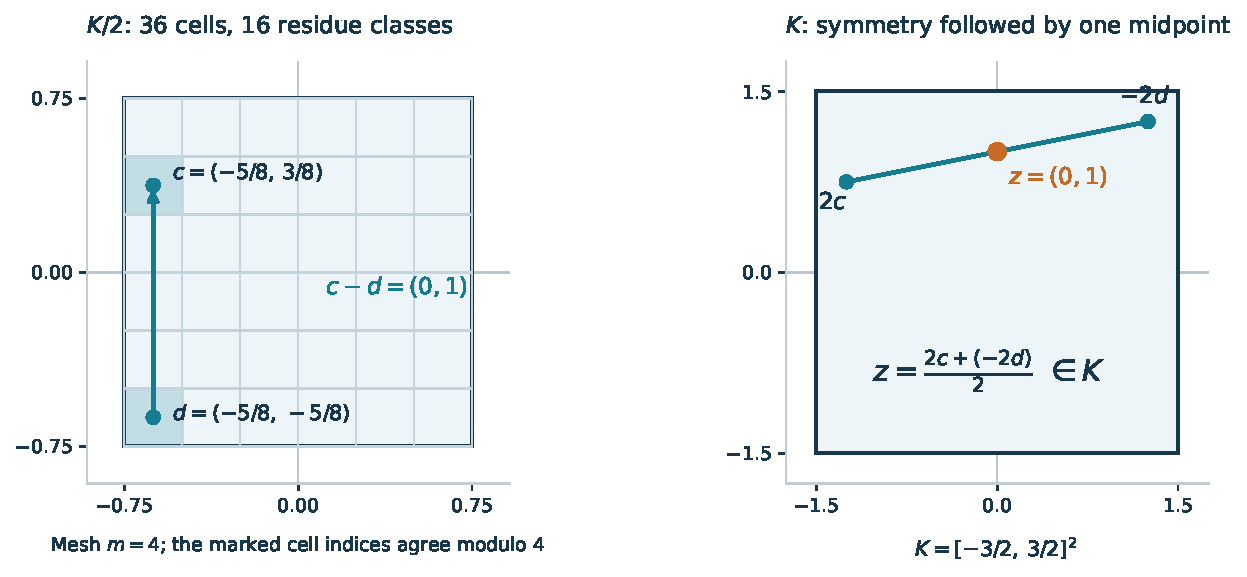
\includegraphics[width=\textwidth]{finite_minkowski.pdf}
\caption{The exact square example. The two selected normalized
centers have an integer difference. Doubling, reflecting one point,
and taking the midpoint places that difference in the original body.}
\label{fig:example}
\end{figure}

\section{Why this is an iPRA proof}\label{sec:audit}

The argument separates arithmetic induction from geometric
membership. This section records the precise audit needed for
the proof-theoretic claim.

\subsection{A fixed correctness equation}

For the rational matrix and slab format, let \(c\) code the
complete finite input. Define fixed primitive recursive functions
\[
                          V(c),\qquad E(c),\qquad G(c,w)
\]
for validation, extraction, and output checking. Invalid
input receives a default output. The uniform arithmetic
theorem is
\begin{equation}\label{eq:object}
 \ipra\vdash\forall c\bigl(V(c)=1\to G(c,E(c))=1\bigr).
\end{equation}
Here \(G\) checks a nonzero integer coefficient vector, its
two contributing cell indices, the scaled-difference
identities, and membership of the returned rational
lattice vector. The witness includes enough data to
verify these claims directly.

For the abstract \(\Phi\) scheme, first prove the purely
arithmetic cell theorem without \(\Phi\). Then instantiate
the two box containment premises and apply symmetry and
midpoint closure once. There is no induction on an
arbitrary body-membership formula and no decision procedure
for it.

\subsection{All required inductions}

\begin{longtable}{L{.25\textwidth}L{.65\textwidth}}
\toprule
Part of the argument & Quantifier-free invariant or identity\\
\midrule
\endhead
Signed quotient/remainder&
\(a=mq+r\) with \(0\leq r<m\), encoded by integer-code equations\\
Mixed-radix enumeration&
Current digits reconstruct the index; digits stay within
their finite coordinate ranges\\
Cell counting&
Prefix count equals the finite sum of products of side widths\\
Disjoint enumeration&
The bounded pairwise-inequality bit is \(1\); a repeated
cell center violates the separating-coordinate check\\
Residue coding&
Partial color equals the partial base-\(m\) sum and is
below \(m^k\); equality is decoded by quotient/remainder\\
Finite pigeonhole&
\(\sum_{r<H}c_r(t)=t\), and the no-repeat bit implies
\(\prod_{r<H}[c_r(t)\leq1]=1\)\\
Nonzero output&
A bounded first-nonzero-coordinate scan; failure means
equality of the two coded vectors\\
Matrix and slab arithmetic&
Finite distributivity and rational cross-multiplication identities\\
\bottomrule
\end{longtable}

These assertions concern finite arrays or explicitly
constructed integers. Every bound in a displayed bounded
quantifier is a primitive recursive term. Replacing that
quantifier by a Boolean fold gives a legitimate induction
instance of \cref{eq:qfind}.

Rational algebra is finite signed-integer algebra with
positive denominators. A displayed division by \(m\) is
justified by \(m\geq1\); a rational inequality can be
multiplied by its positive denominator. The identity
\cref{eq:cell-count} needs only finite products, finite
sums, and distributivity. The geometric last step uses
equality replacement, implication elimination, and
conjunction; it has no inductive content.

\subsection{Explicit bounds}

Let \(D_0\) be the product of all endpoint denominators.
We may use \(m=D_0\), or compute a smaller common multiple.
For a valid certificate,
\begin{align*}
 &m\leq D_0,\qquad H=m^n,\\
 &\text{cells required by the extractor}\leq H+1,\\
 &\text{pairs in a direct collision search}\leq H(H+1)/2,\\
 &\text{color-table slots}=H.
\end{align*}
Each cell is decoded with at most \(s\) prefix comparisons
and \(n\) mixed-radix operations. If every box lies in
\([-R,R]^n\), then its centers do too, so
\begin{equation}\label{eq:coefficient-bound}
                              \norminf{z}\leq2R.
\end{equation}

The sequence encodings have primitive recursive bounds as
well. An array of length \(L\) whose entries are below \(M\)
can be encoded in base \(M+1\) below \((M+1)^L\), together
with its length and base. Signed coordinates and rational
pairs admit the same kind of bound after their components
are bounded. Bounded iteration of a coded state is ordinary
primitive recursion. No claim here is polynomial-time:
the purpose is the proof-theoretic bound, not efficient
lattice reduction.
